\documentclass[12pt]{article}
\usepackage[margin=2.5cm]{geometry}
\usepackage{enumerate}
\usepackage{amsfonts}
\usepackage{amsmath}
\usepackage{fancyhdr}
\usepackage{amsmath}
\usepackage{amssymb}
\usepackage{amsthm}
\usepackage{mdframed}
\usepackage{graphicx}
\usepackage{subcaption}
\usepackage{adjustbox}
\usepackage{listings}
\usepackage{xcolor}
\usepackage{booktabs}
\usepackage[utf]{kotex}
\usepackage{hyperref}

\definecolor{codegreen}{rgb}{0,0.6,0}
\definecolor{codegray}{rgb}{0.5,0.5,0.5}
\definecolor{codepurple}{rgb}{0.58,0,0.82}
\definecolor{backcolour}{rgb}{0.95,0.95,0.92}

\lstdefinestyle{mystyle}{
    backgroundcolor=\color{backcolour},
    commentstyle=\color{codegreen},
    keywordstyle=\color{magenta},
    numberstyle=\tiny\color{codegray},
    stringstyle=\color{codepurple},
    basicstyle=\ttfamily\footnotesize,
    breakatwhitespace=false,
    breaklines=true,
    captionpos=b,
    keepspaces=true,
    numbers=left,
    numbersep=5pt,
    showspaces=false,
    showstringspaces=false,
    showtabs=false,
    tabsize=1
}

\lstset{style=mystyle}

\pagestyle{fancy}
\renewcommand{\headrulewidth}{0.4pt}
\lhead{Hyungmo Gu}
\rhead{CSC369 Week 3 Notes}

\begin{document}
\title{CSC369 Week 3 Notes}
\author{Hyungmo Gu}
\maketitle

\bigskip

\section{Synchronization}

\bigskip
\begin{itemize}
    \item Producer and Consumer Problem
    \begin{itemize}
        \item Is also known as \textbf{bound-and-buffer} problem
        \item Achieves synchronization
        \item Has two types of processes
        \begin{enumerate}[1.]
            \item \textbf{Producer}
            \begin{itemize}
                \item Produces data
                \item Puts data into buffer
            \end{itemize}
            \item \textbf{Consumer}
            \begin{itemize}
                \item Consumes data
                \item Removes data from buffer, one piece at a time
            \end{itemize}
        \end{enumerate}
        \item It's like kimchi factory, or delicious cookie factory :)

        \begin{center}
        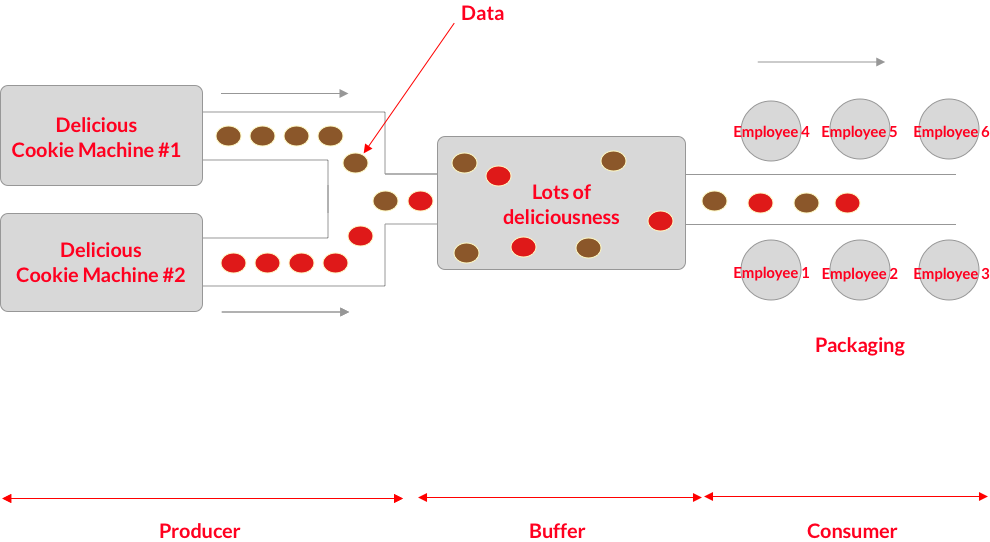
\includegraphics[width=\linewidth]{images/week_3_notes_1_1.png}
        \end{center}
    \end{itemize}

    \item Semaphore
    \begin{itemize}
        \item Developed by Dijkstra in 1962.
        \item Provides synchronization
        \item Works like a signal
        \begin{itemize}
            \item Uses a non-negative integer variable that is shared between threads
            \item Has two ``\textbf{atomic}'' operations
            \begin{enumerate}[1.]
                \item \textbf{Wait} (Also called P, or decrement)
                \item \textbf{Signal} (Also called V, or increment)
            \end{enumerate}
        \end{itemize}
    \end{itemize}
\end{itemize}

\bigskip



\end{document}